\question A group of students takes CSM mock final. After the exam, each student is told his or her percentile rank among all students taking the exam. 

\begin{enumerate}[label=(\alph*)] 
\item If a student is randomly picked, what is the probability that the student's percentile rank is over 70\%? 
\begin{solution}[4cm] 
Let X be the percentile rank of the student. Then X is a random variable uniformly distributed between 0 and 1. Thus, $P(X > 0.7) = 0.3$. 
\end{solution}

\item If two students are picked independently at random, what is the probability that their percentile ranks differ by more than 10\%? (Hint: draw a diagram to determine the region of the event) 
\begin{solution}[4cm]
Let $X$ be the percentile rank of the first student, and $Y$ be the percentile rank of the second student. Since $X$ and $Y$ are two independent uniform(0, 1) random variable, we know the joint density of $X, Y$ is $f_{X, Y} (x, y) = 1$. The event that \{two ranks differ by more than 10\%\} is equivalent to $|X - Y| > 0.1$, which region is denoted by the shaded area in the following diagram: \\ 

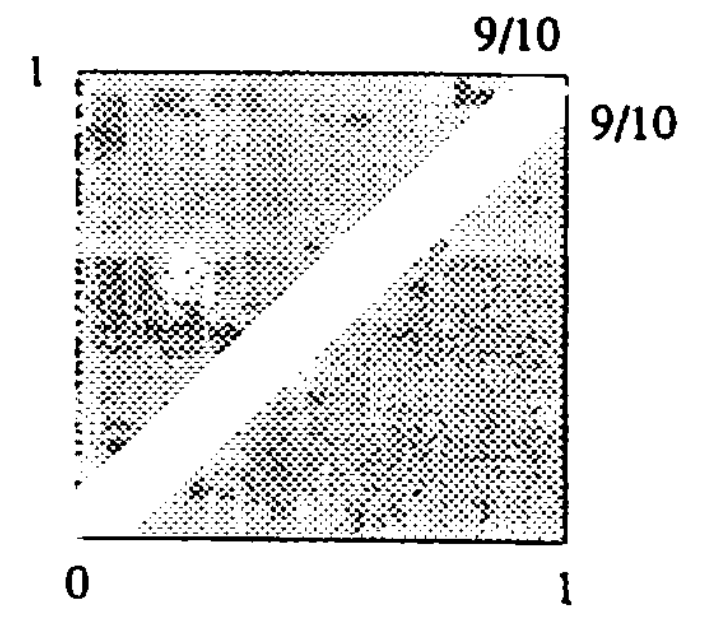
\includegraphics[width=2in]{density.png} 

Thus, $P(|X - Y| > 0.1) = 2 \times \frac{1}{2} \frac{9}{10} ^ 2 = 0.81$. 

\end{solution}
\end{enumerate}